% Preamble templated from Mihir-Divyansh/Course-Setup
%iffalse
\let\negmedspace\undefined
\let\negthickspace\undefined
\documentclass[journal,12pt,onecolumn]{IEEEtran}
\usepackage{cite}
\usepackage{amsmath,amssymb,amsfonts,amsthm}
\usepackage{algorithmic}
\usepackage{graphicx}
\usepackage{textcomp}
\usepackage{xcolor}
\usepackage{txfonts}
\usepackage{listings}
\usepackage{enumitem}
\usepackage{mathtools}
\usepackage{gensymb}
\usepackage{comment}
\usepackage[breaklinks=true]{hyperref}
\usepackage{tkz-euclide}
\usepackage{listings}
\usepackage{gvv}
%\def\inputGnumericTable{}
\usepackage[latin1]{inputenc}
\usepackage{color}
\usepackage{array}
\usepackage{longtable}
\usepackage{calc}
\usepackage{multirow}
\usepackage{hhline}
\usepackage{ifthen}
\usepackage{lscape}
\usepackage{tabularx}
\usepackage{array}
\usepackage{float}
\usepackage{caption}
\usepackage{multicol}

\newtheorem{theorem}{Theorem}[section]
\newtheorem{problem}{Problem}
\newtheorem{proposition}{Proposition}[section]
\newtheorem{lemma}{Lemma}[section]
\newtheorem{corollary}[theorem]{Corollary}
\newtheorem{example}{Example}[section]
\newtheorem{definition}[problem]{Definition}
\newcommand{\BEQA}{\begin{eqnarray}}
\newcommand{\EEQA}{\end{eqnarray}}
%\newcommand{\define}{\stackrel{\triangle}{=}}
\theoremstyle{remark}
%\newtheorem{rem}{Remark}

% Marks the beginning of the document
\begin{document}
\bibliographystyle{IEEEtran}
\vspace{3cm}

\title{Assignment 7: 4.7.52}
\author{EE25BTECH11055 - Subhodeep Chakraborty}
\maketitle
\hrulefill
\bigskip

\renewcommand{\thefigure}{\theenumi}
\renewcommand{\thetable}{\theenumi}

\textbf{Question:}\par
If the points \brak{1, 1, p} and \brak{-3, 0, 1} be equidistant from the plane $\vec{r}\cdot\brak{3\hat{\imath} + 4\hat{\jmath} -12\hat{k}}+13=0$, then find the value of $p$.
\par
\textbf{Solution:}\par

Given:
\begin{align}
 \vec{A} &= \myvec{1\\1\\p} \\
 \vec{B} &= \myvec{-3\\0\\1}\\
 \myvec{3 & 4 & -12}\vec{r} &= -13
\end{align}

We know,
\begin{align}
 d = \frac{|\vec{n}^\top\vec{P}-c|}{\norm{\vec{n}}}
\end{align}
Thus
\begin{align}
 \frac{|\vec{n}^\top\vec{A}-c|}{\norm{\vec{n}}} &= \frac{|\vec{n}^\top\vec{B}-c|}{\norm{\vec{n}}} \\
 \vec{n}^\top\vec{A} = \vec{n}^\top\vec{B} &\text{ OR } \vec{n}^\top\vec{A} = 2c - \vec{n}^\top\vec{B}
\end{align}
Substituting values
\begin{align}
7 - 12p = -21 &\textbf{  OR  } 7-12p = -26 + 21 \\
p = 7/3 &\textbf{  OR  } p = 1
\end{align}
\begin{figure}[H]
    \centering
    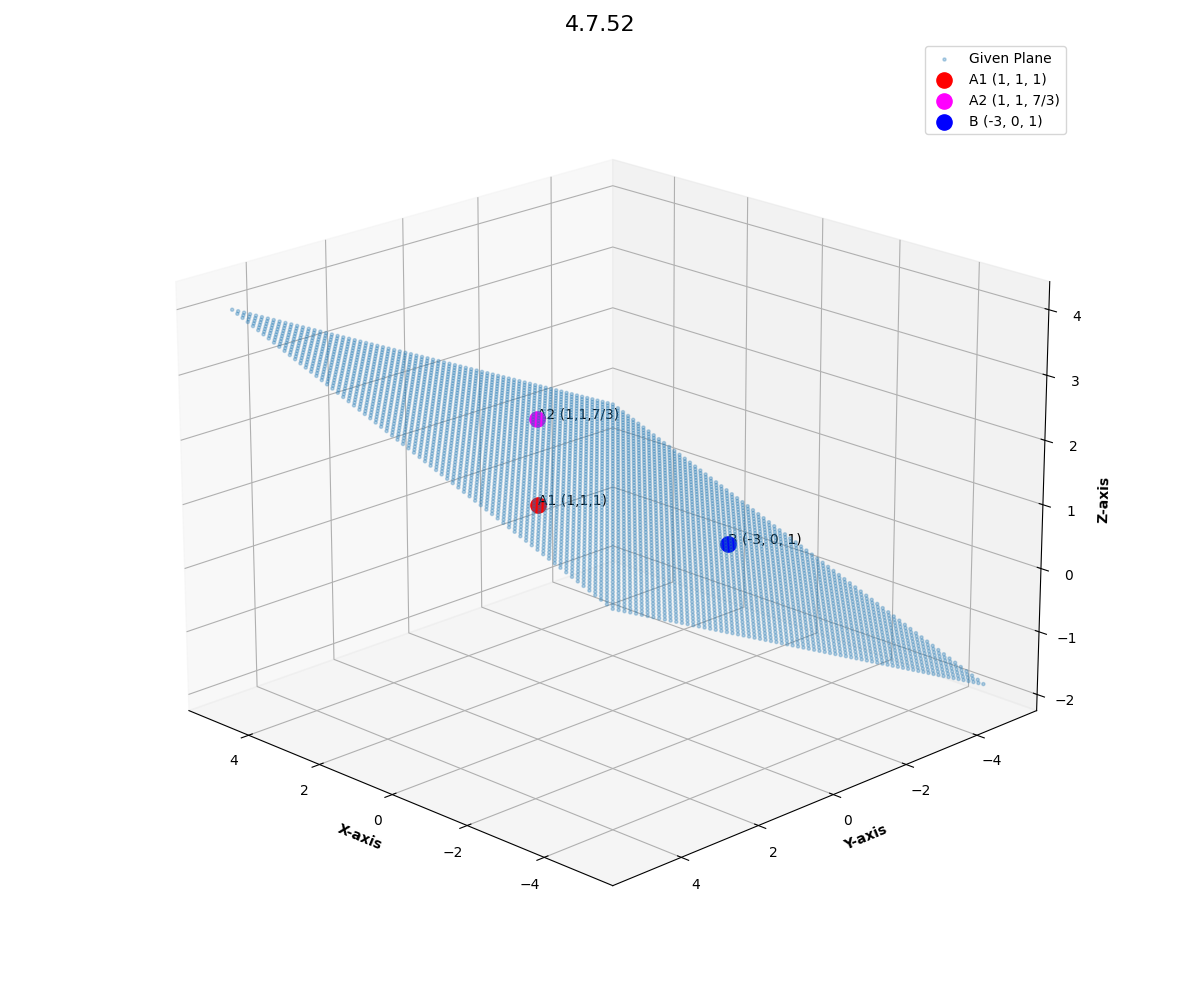
\includegraphics{figs/plot.png}
    \caption*{}
    \label{fig:plot}
\end{figure}
\end{document}
